% Provisional study timeline (Gantt-style chart), October 2026 to April 2027.
% Category palette: proposal (gray), data (blue), experiments (teal),
% integration (violet), writing (amber); dissemination reuses the writing hue.
\definecolor{gFill}{RGB}{226,232,240}
\definecolor{gDraw}{RGB}{51,65,85}
\definecolor{bFill}{RGB}{219,234,254}
\definecolor{bDraw}{RGB}{30,64,175}
\definecolor{tFill}{RGB}{204,251,241}
\definecolor{tDraw}{RGB}{15,118,110}
\definecolor{pFill}{RGB}{237,233,254}
\definecolor{pDraw}{RGB}{91,33,182}
\definecolor{aFill}{RGB}{254,243,199}
\definecolor{aDraw}{RGB}{146,64,14}

% Legend entry: a rounded color swatch (fill/draw) followed by its label.
\newcommand{\lgitem}[3]{%
  \tikz[baseline=-0.5ex]{\draw[fill=#1,draw=#2,rounded corners=1pt,line width=0.4pt]
    (0,0) rectangle (0.26,0.26);}\,#3}

% Body font is Palatino (mathpazo), the Book Antiqua-compatible face used by
% the manuscript; \normalfont keeps labels upright in that same family.
\begin{figure}[t]
\centering
\resizebox{0.8\textwidth}{!}{%
\begin{tabular}{@{}c@{}}
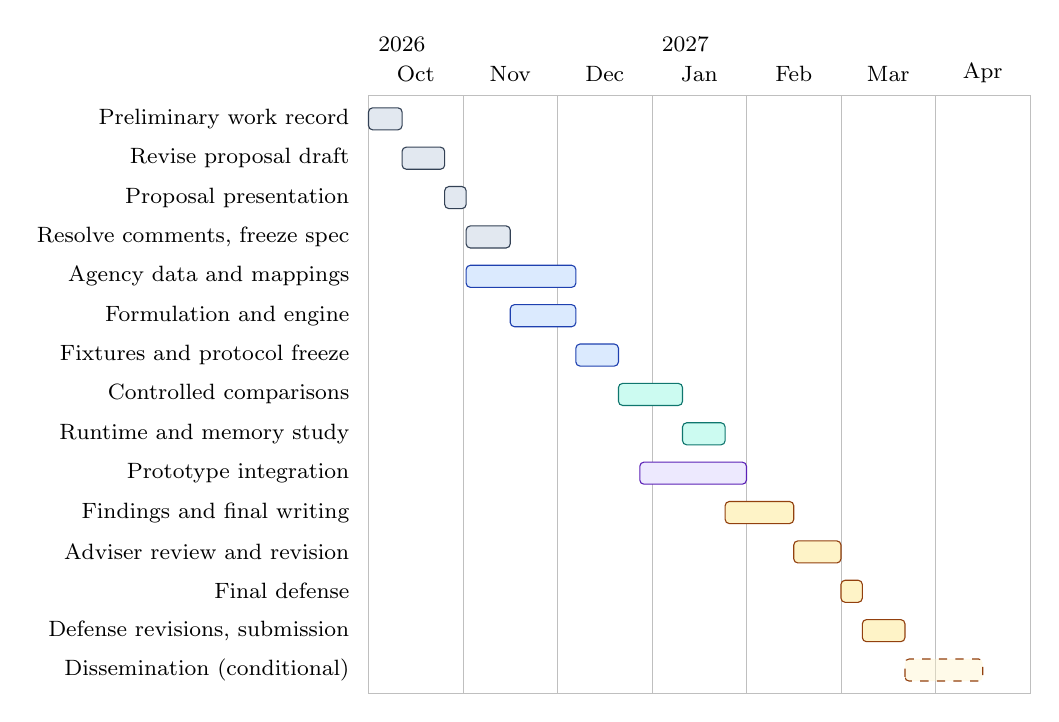
\begin{tikzpicture}[
  x=1.2cm, y=0.5cm, font=\normalfont\footnotesize,
  proposal/.style={fill=gFill, draw=gDraw, rounded corners=1.5pt, line width=0.4pt},
  data/.style={fill=bFill, draw=bDraw, rounded corners=1.5pt, line width=0.4pt},
  exper/.style={fill=tFill, draw=tDraw, rounded corners=1.5pt, line width=0.4pt},
  integ/.style={fill=pFill, draw=pDraw, rounded corners=1.5pt, line width=0.4pt},
  write/.style={fill=aFill, draw=aDraw, rounded corners=1.5pt, line width=0.4pt},
  disem/.style={fill=aFill, fill opacity=0.4, draw=aDraw, dashed,
                rounded corners=1.5pt, line width=0.4pt},
  grid/.style={draw=black!25, line width=0.3pt}
]

% Bar macro: {row}{start}{end}{style}{label}  (start/end in months from 1 Oct 2026)
\newcommand{\gbar}[5]{%
  \node[anchor=east] at (-0.1,-#1) {#5};
  \draw[#4] (#2,-#1-0.28) rectangle (#3,-#1+0.28);}

% Grid and axis
\foreach \m in {0,...,7}{\draw[grid] (\m,0.6) -- (\m,-14.6);}
\draw[grid] (0,0.6) -- (7,0.6);
\draw[grid] (0,-14.6) -- (7,-14.6);
\node[anchor=west] at (0,1.9) {2026};
\node[anchor=west] at (3,1.9) {2027};
\foreach \m/\n in {0/Oct,1/Nov,2/Dec,3/Jan,4/Feb,5/Mar,6/Apr}{
  \node at (\m+0.5,1.15) {\n};}

% Activities
\gbar{0}{0}{0.355}{proposal}{Preliminary work record}
\gbar{1}{0.355}{0.806}{proposal}{Revise proposal draft}
\gbar{2}{0.806}{1.033}{proposal}{Proposal presentation}
\gbar{3}{1.033}{1.500}{proposal}{Resolve comments, freeze spec}
\gbar{4}{1.033}{2.194}{data}{Agency data and mappings}
\gbar{5}{1.500}{2.194}{data}{Formulation and engine}
\gbar{6}{2.194}{2.645}{data}{Fixtures and protocol freeze}
\gbar{7}{2.645}{3.323}{exper}{Controlled comparisons}
\gbar{8}{3.323}{3.774}{exper}{Runtime and memory study}
\gbar{9}{2.871}{4.000}{integ}{Prototype integration}
\gbar{10}{3.774}{4.500}{write}{Findings and final writing}
\gbar{11}{4.500}{5.000}{write}{Adviser review and revision}
\gbar{12}{5.000}{5.226}{write}{Final defense}
\gbar{13}{5.226}{5.677}{write}{Defense revisions, submission}
\gbar{14}{5.677}{6.500}{disem}{Dissemination (conditional)}

\end{tikzpicture}\\[9pt]

% Centered legend, matching the chart palette.
{\footnotesize
\begin{tabular}{@{}c@{}}
\lgitem{gFill}{gDraw}{Proposal}\hspace{1.6em}%
\lgitem{bFill}{bDraw}{Data and engine}\hspace{1.6em}%
\lgitem{tFill}{tDraw}{Experiments}\\[3pt]
\lgitem{pFill}{pDraw}{Integration}\hspace{1.6em}%
\lgitem{aFill}{aDraw}{Writing and defense}
\end{tabular}}
\end{tabular}%
}

\caption{Planned schedule, October 2026 to April 2027.}
\label{fig:timeline}
\end{figure}
